\documentclass{article}
\usepackage{graphicx} % Required for inserting images
\usepackage{kotex}
\usepackage{listings}
\usepackage{geometry}
\usepackage{xcolor}
\usepackage{verbatim}
\usepackage{indentfirst}

\renewcommand{\figurename}{그림}

\geometry{
    a4paper,
    left=30mm,
    right=30mm,
    top=30mm,
    bottom=40mm
}

\lstset{language=C++,
            basicstyle=\ttfamily,
            keywordstyle=\color{blue}\ttfamily,
            stringstyle=\color{red}\ttfamily,
            commentstyle=\color{teal}\ttfamily,
            numberstyle=\tiny\color{gray}\ttfamily,
            morecomment=[l][\color{magenta}]{\#}
            breakatwhitespace=false,         
            breaklines=true,                 
            captionpos=b,                    
            keepspaces=true,                 
            numbers=left,                    
            numbersep=5pt,                  
            showspaces=false,                
            showstringspaces=false,
            showtabs=false,                  
            tabsize=2
}

\title{객체지향프로그래밍 \\
\large HW03}
\author{C211123 이준선}
\date{2023년 3월 16일}

\begin{document}

\maketitle

\section{코드}

\begin{lstlisting}[language=C++, escapeinside=``, caption=main.cpp, label={lstlisting:main.cpp}]
#include <iostream>
#include <ctime>
#include <cstdlib>
#include <random>

/// @brief uniform distributed random even number generator
class EvenRandom
{
public:
    /// @brief seed `설정`
    EvenRandom();

    /// @brief `랜덤 짝수 리턴`
    /// @return random even number
    int next();

    /// @brief `low와 high 사이의 랜덤 짝수 리턴`
    /// @param low minimum value
    /// @param high maximum value
    /// @return [low, high] `사이의 랜덤 짝수`
    int nextInRange(const int low, const int high);

private:
    std::random_device random_device;
    std::mt19937 mt_engine;
    std::uniform_int_distribution<int> uniform_distributor;
};

EvenRandom::EvenRandom()
    : mt_engine(random_device())
{
    // `최대 분포를 RAND\_MAX의 절반으로 설정 (결과값에 * 2를 하기 위함)`
    uniform_distributor.param(std::uniform_int_distribution<int>::param_type(0, RAND_MAX / 2));
}

int EvenRandom::next()
{
    return uniform_distributor(mt_engine) * 2;
}

int EvenRandom::nextInRange(const int low, const int high) 
{
    std::uniform_int_distribution<int> ranged_distributor(low / 2, high / 2);
    return ranged_distributor(mt_engine) * 2;
}

int main()
{
    EvenRandom r;
    std::cout << "-- 0`에서` " << RAND_MAX << "`까지의 랜덤 짝수 정수 10 개`--" << std::endl;
    for (int i = 0; i < 10; i++)
    {
        int n = r.next(); // `0에서 RAND\_MAX(32767) 사이의 랜덤한 정수`
        std::cout << n << ' ';
    }
    std::cout << std::endl
              << std::endl
              << "-- 2`에서` "
              << "10 `까지의 랜덤 짝수 정수 10 개` --" << std::endl;
    for (int i = 0; i < 10; i++)
    {
        int n = r.nextInRange(2, 10); // `2에서 10 사이의 랜덤한 정수`
        std::cout << n << ' ';
    }
    std::cout << std::endl;
}
\end{lstlisting}

코드 \ref{lstlisting:main.cpp}의 raw format 버전은 본 문서 아래에 담아놨음.

\newpage
\section{결과}
\begin{figure}[ht]
    \centering
    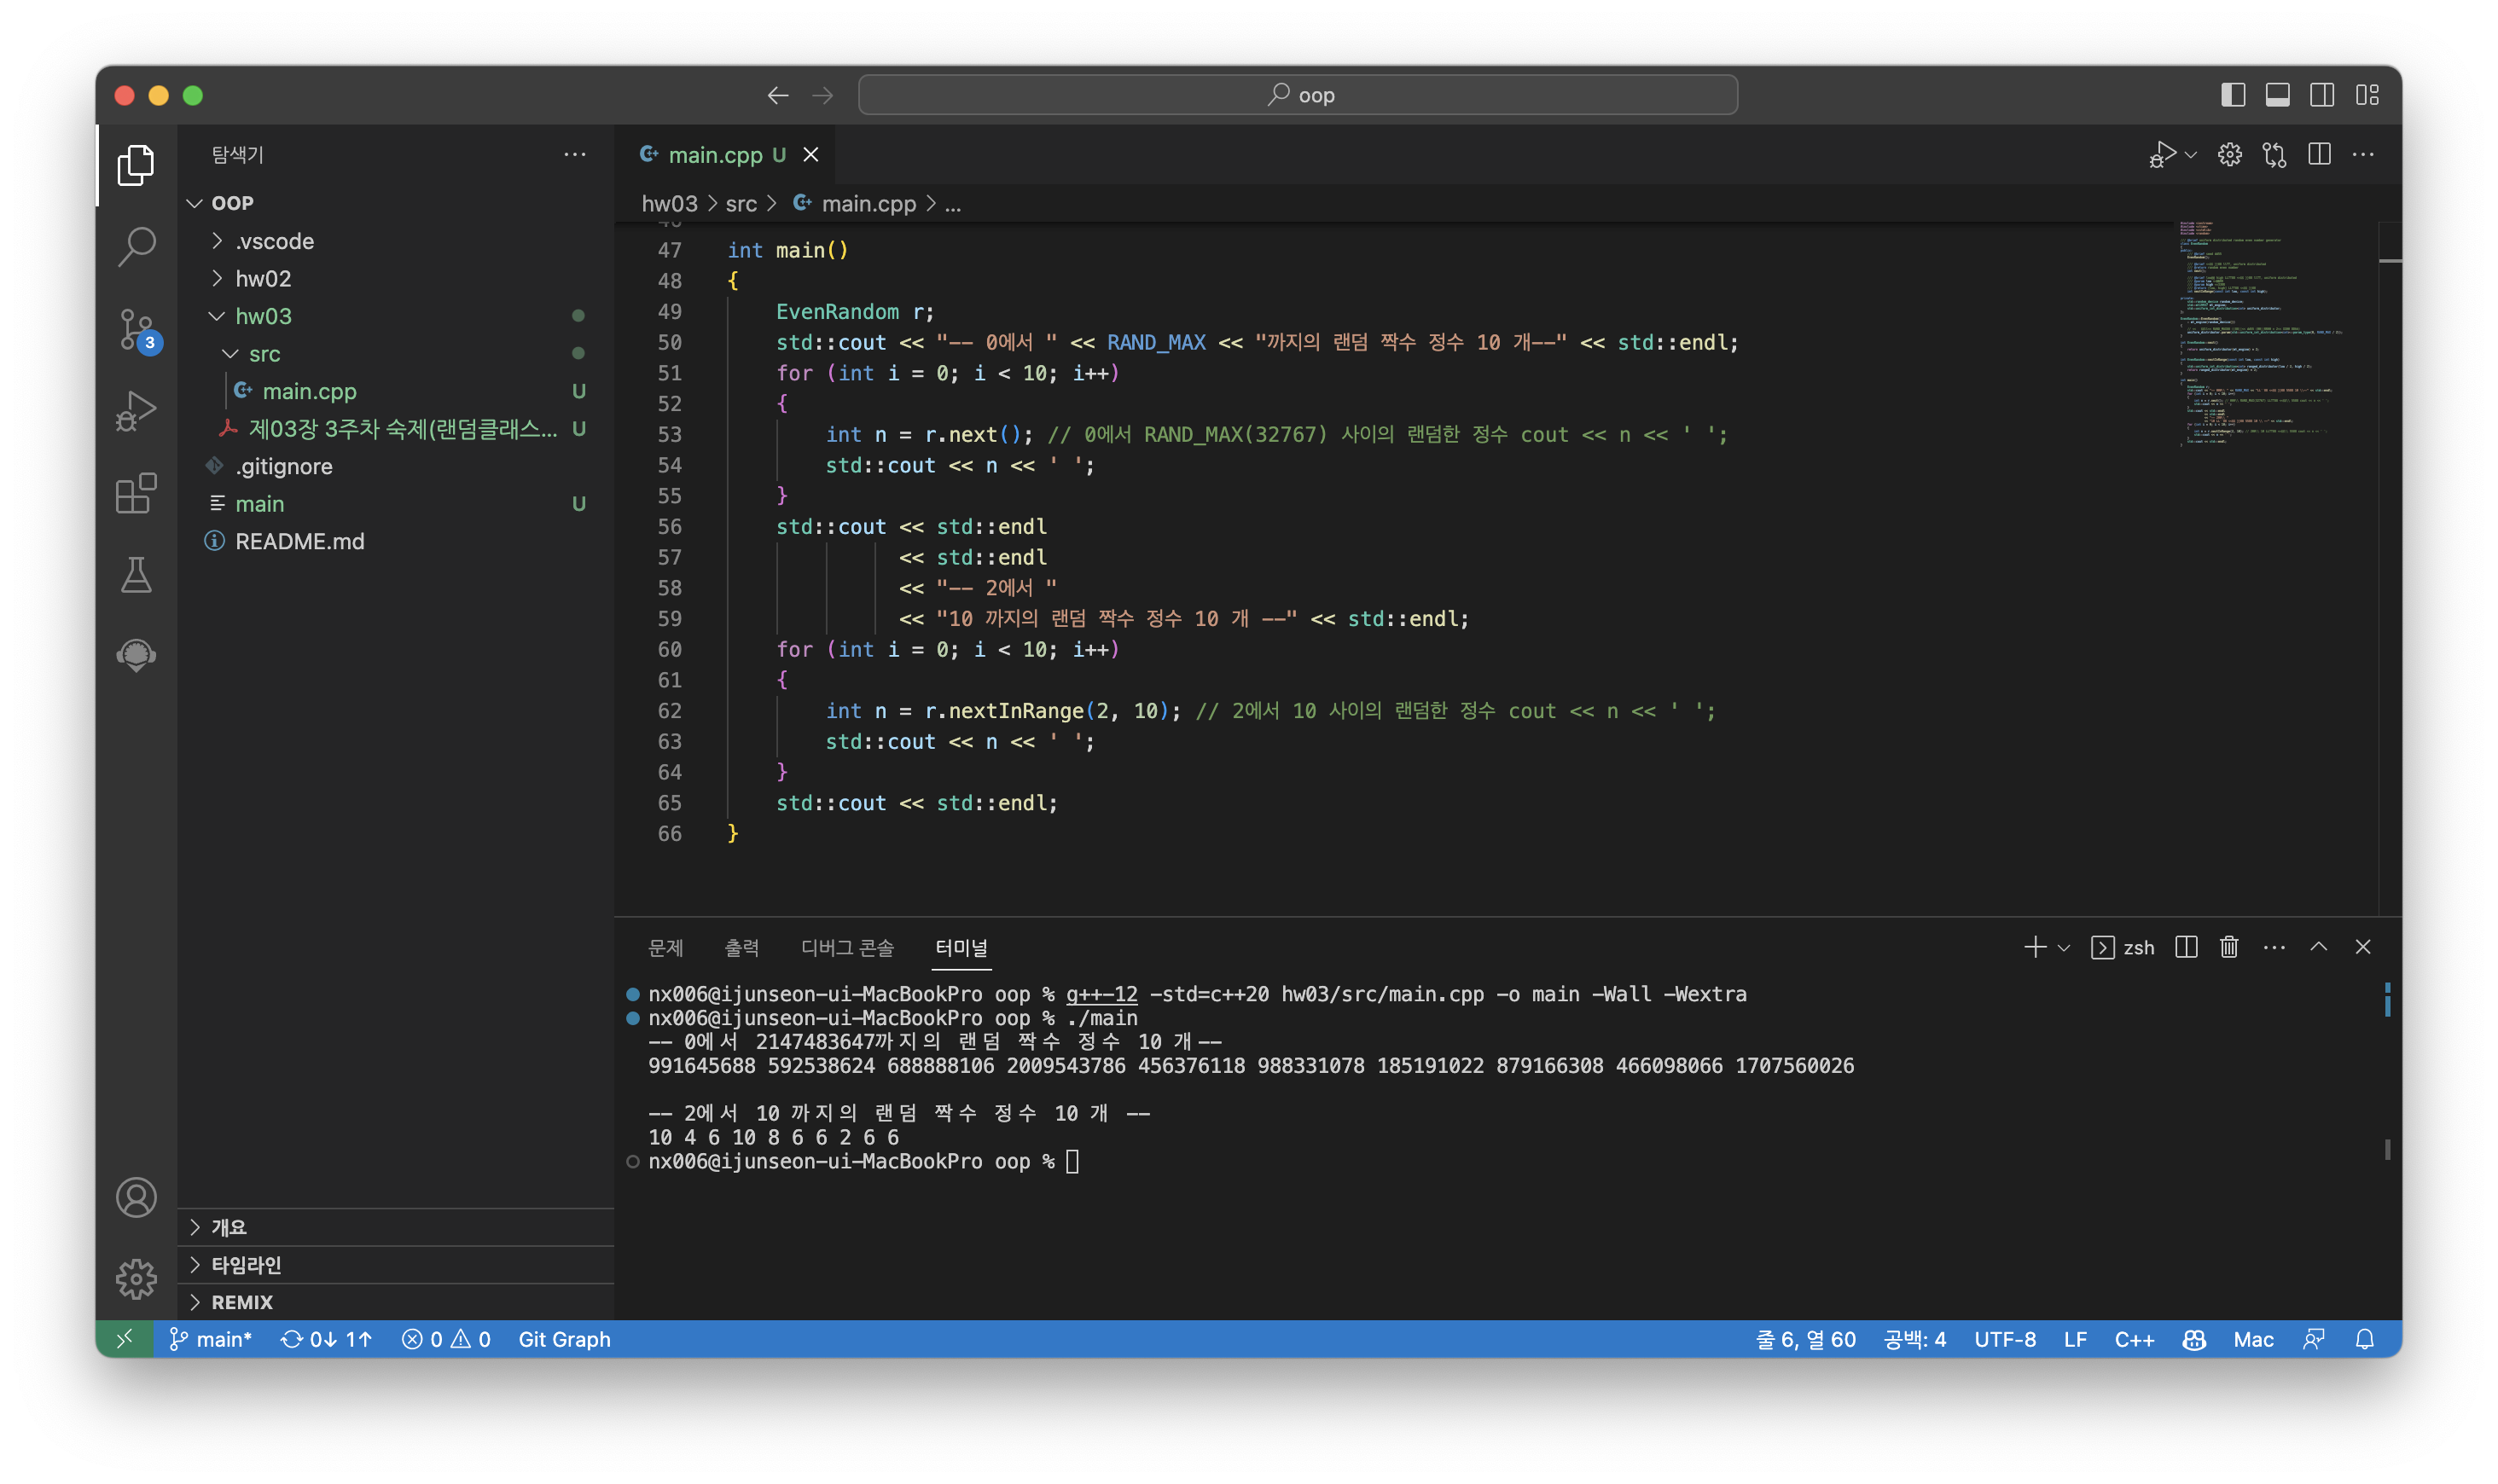
\includegraphics[width=\textwidth]{random_result.png}
    \caption{실행 결과}
    \label{fig:result}
\end{figure}

\newpage
\section{참고}
random 헤더는 C++11부터 도입됐기 때문에 컴파일러 옵션에 -std=c++11, 혹은 그 이상의 버전을 붙여주어야 한다.

그림 \ref{fig:result}에서 최댓값이 2147483647로 설정됐다. 과제 명세서에 적힌 값과 다른데, 컴파일러 혹은 C++ 버전에 따라 RAND\_MAX의 값은 달라질 것이므로 이를 굳이 수정하지는 않았다.
C++버전은 C++20, 컴파일러는 g++-12 버전을 사용했다.

\begin{figure}
    \centering
    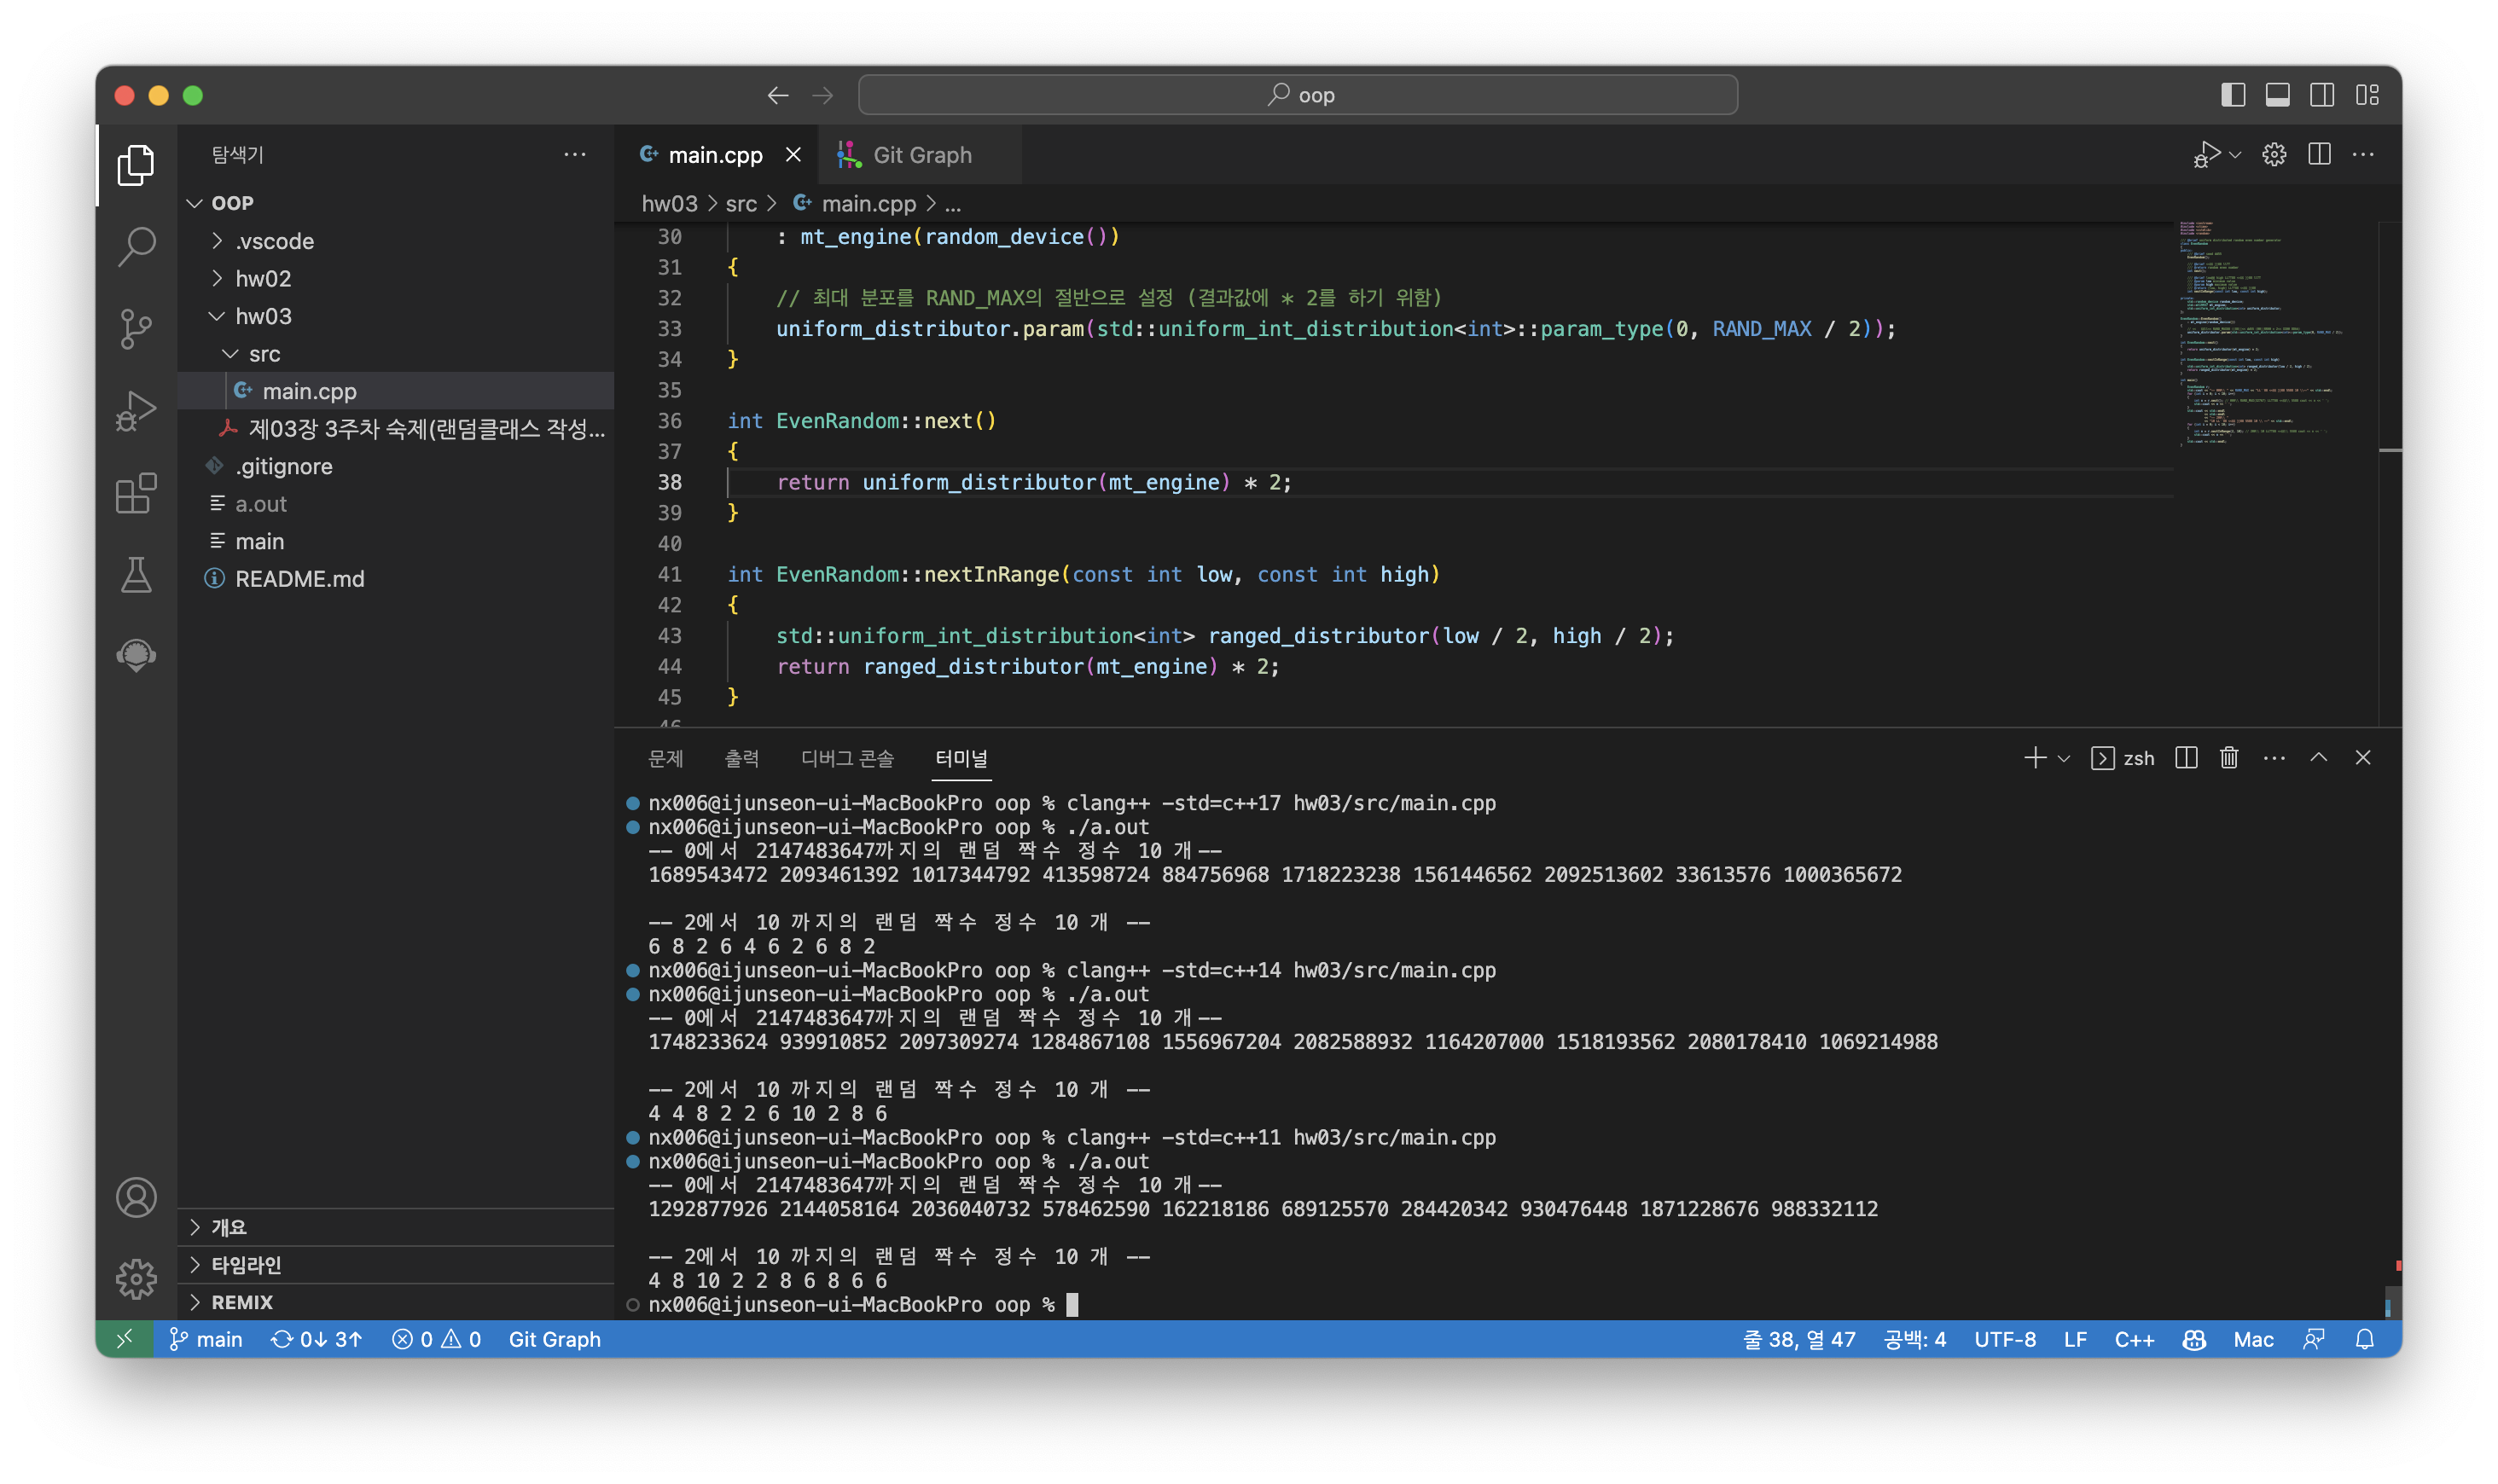
\includegraphics[width=\textwidth]{clang_result.png}
    \caption{Clang result}
    \label{fig:clang result}
\end{figure}

사실 컴파일러를 g++이 아닌 clang으로 바꾸고, C++ 버전을 11, 14, 17로 바꾸어도 과제 명세서에 적힌 값은 얻을 수 없었다(그림 \ref{fig:clang result}). 이는 애초에 cstdlib 에서 매크로로 정의된 RAND\_MAX의 값이 0x7fffffff로 int 범위의 최댓값(약 21억)으로 정의됐기 때문이다.

\newpage
\section{코드(RAW)}
\thispagestyle{empty}

코드 \ref{lstlisting:main.cpp}의 raw format 버전을 아래 담았다.

\begin{verbatim}
#include <iostream>
#include <ctime>
#include <cstdlib>
#include <random>

/// @brief uniform distributed random even number generator
class EvenRandom
{
public:
    /// @brief seed 설정
    EvenRandom();

    /// @brief 랜덤 짝수 리턴
    /// @return random even number
    int next();

    /// @brief low와 high 사이의 랜덤 짝수 리턴
    /// @param low minimum value
    /// @param high maximum value
    /// @return [low, high] 사이의 랜덤 짝수
    int nextInRange(const int low, const int high);

private:
    std::random_device random_device;
    std::mt19937 mt_engine;
    std::uniform_int_distribution<int> uniform_distributor;
};

EvenRandom::EvenRandom()
    : mt_engine(random_device())
{
    // 최대 분포를 RAND_MAX의 절반으로 설정 (결과값에 * 2를 하기 위함)
    uniform_distributor.param(std::uniform_int_distribution<int>::param_type(0, RAND_MAX / 2));
}

int EvenRandom::next()
{
    return uniform_distributor(mt_engine) * 2;
}

int EvenRandom::nextInRange(const int low, const int high) 
{
    std::uniform_int_distribution<int> ranged_distributor(low / 2, high / 2);
    return ranged_distributor(mt_engine) * 2;
}

int main()
{
    EvenRandom r;
    std::cout << "-- 0에서 " << RAND_MAX << "까지의 랜덤 짝수 정수 10 개--" << std::endl;
    for (int i = 0; i < 10; i++)
    {
        int n = r.next(); // 0에서 RAND_MAX(32767) 사이의 랜덤한 정수 cout << n << ' ';
        std::cout << n << ' ';
    }
    std::cout << std::endl
              << std::endl
              << "-- 2에서 "
              << "10 까지의 랜덤 짝수 정수 10 개 --" << std::endl;
    for (int i = 0; i < 10; i++)
    {
        int n = r.nextInRange(2, 10); // 2에서 10 사이의 랜덤한 정수 cout << n << ' ';
        std::cout << n << ' ';
    }
    std::cout << std::endl;
}
\end{verbatim}

\end{document}
